\documentclass[headinclude, footinclude, abstract=on]{scrarticle}
\usepackage[left=1in, right=1in, top=1in, bottom=1in]{geometry}
\usepackage{graphicx} % Required for inserting images
\usepackage{hyperref}
\usepackage{minted}
\usepackage{longtable}
\graphicspath{ {./images/} }
\usepackage{algorithm}
\usepackage{algpseudocode}
\usepackage{titling}
\usepackage{courier}
\usepackage{geometry}
\usepackage{multirow}
 \geometry{
 a4paper,
 total={170mm,257mm},
 left=15mm,
 top=15mm,
 }
\bibliographystyle{plain} % We choose the "plain" reference style

\pretitle{\begin{centering}\Huge\bfseries}
\posttitle{\par\end{centering}\vskip 0.5em}
\preauthor{\begin{center}\Large\ttfamily}
\postauthor{\end{center}}
\predate{\par\large\centering}
\postdate{\par}

\title{\normalfont\spacedallcaps{ANSWER SET AND \\ CONSTRAINT PROGRAMMING}}
\author{\spacedlowsmallcaps{ZANOLIN LORENZO}}

\date{}

\begin{document}
\maketitle
\thispagestyle{empty}

\begin{abstract}
COP (Constraint Optimization Problem) are problems for which we want to find an assignment for the variables in order to satisfy some \textit{constraints} and also to minimize a \textit{cost function}. The aim of this report is to solve a COP problem using \textit{Constraint Programming} and \textit{Answer Set Programming} and compare measured performances. 
\end{abstract}

\tableofcontents
\clearpage
\section{Introduction}
The objective of this activity is to compare different modelling techniques for a COP problem. Specifically, we will consider the \textit{MiniZinc} constraint modeling language and the \textit{ASP programming paradigm} (using the Clingo answer set solver). For each system, we will present the modeling of the general problem, showing how each constraint of the assignment can be implemented. Subsequently, we will present a Python script to generate pseudo-random instances with increasing complexity and finally we will propose some performance metrics of the two solvers on these test cases.

\subsection{Problem description}
The problem is similar to the famous \textit{Sokoban Problem}~\cite{sok,dovier}.
We need to move $k$ boxes $b_1,\cdots,b_k$, whose size is $s_1,\cdots,s_k$, inside a $m \times n$ room. The aim is to stack all boxes at the bottom starting from the left corner using the minimum number of moves. If there is not enough space at the bottom, the worker will stack them higher until there is enough space.The only available move is \textit{move(i,d)} which push the $b_i$ box towards direction $d$.

\subsubsection{Constraints}
We consider two kinds of constraints:
\begin{itemize}
    \item \textit{Hard} Constraints: those which must be always satisfied.
    In this case we consider:
        \begin{itemize}
            \item \textit{Push}: only \textit{pushing} is allowed, worker cannot \textit{pull} boxes;
            \item \textit{Pushable}: to push a box, there must be \textit{at least} an empty space in front of the box (where the worker is);
            \item \textit{Free Row}: to push a box, \textit{all} cells beyond the box (towards decided direction $d$) must be empty;
            \item \textit{Inertia}: if a box is not pushed at time $t_i$, then it must be at the same position at time ${t}_{i+1}$;
            \item \textit{Move}: only a move at time is accepted.
        \end{itemize}
        
    \item \textit{Soft} Constraints: those which aren't strictly necessary, but is better to have them satisfied:
    \begin{itemize}
        \item \textit{Number of moves}: number of moves has to be minimum;
    \end{itemize}
\end{itemize}

An example of the problem is represented in figure~\ref{fig:set}. The left part is the initial state while the right one is the final state, in which all boxed are stacked correctly. 
\begin{figure}[ht]
	\centering
	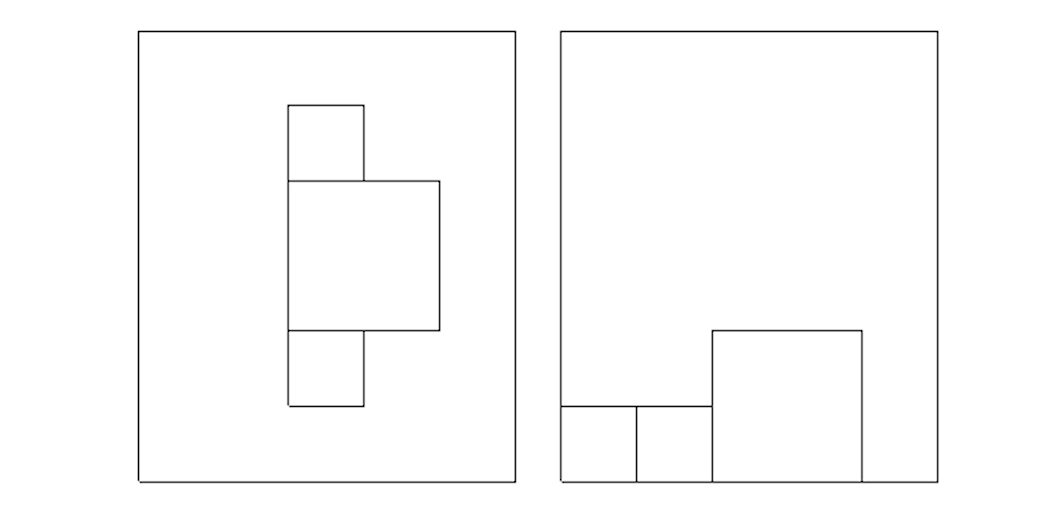
\includegraphics[width=0.5\textwidth]{images/set.png}
    \caption{Initial and final state of the problem.}
    \label{fig:set}
\end{figure}

\subsubsection{Cost function}The approach taken in the two solution is slightly different. As we will see, in the \textit{ASP} setting we considered the \textit{number of moves} as a function and the aim is to find global \textit{minimum} of it; while in the \hyperref[sec:mzn]{\textit{CP}} one we considered the \textit{number of null moves} as a function and the aim is to find a global \textit{maximum} of it.

\subsubsection{Assumptions} The following choices were made:
\begin{itemize}
    \item We start stacking bigger boxes in the left corner, so they are always at the leftmost part of the room.  
    \item For simplicity we do not consider sokoban movements, anyway we consider that the cell were the sokoban should be must be empty.  
\end{itemize}
%\vfill
%\clearpage
\section{MiniZinc Modelling}\label{sec:mzn}
The following \textit{model} is composed of 4 parts, we will briefly analyze all of them.

\subsection{Variables definition}
We use the following variables, which are given in input from instances, to model the problem:
\begin{minted}[frame=single]{prolog}
int: n;  % height of the room
int: m;  % base of the room
int: k;  % number of cartons, each of them is a square of size s_k
int: maxTime; % maximum number of steps
int: maxDim;  % maximum size of a carton
\end{minted}
\\
With the previous variables, we can the define sets that we will use as sizing for arrays.
\begin{minted}[frame=single]{prolog}
set of int: STEPS = 1..maxTime-1;
set of int: CARTONS = 1..k;
set of int: ROWS = 1..n;
set of int: COLUMNS = 1..m;
set of int: SIZE = 1..maxDim;
set of int: MOVES = {0,1,2,3,4};  
\end{minted}
A \textit{move} is represented using numbers, in this case: 0:DOWN  1:UP  2: LEFT  3:RIGHT  4:NONE
\\
Finally, we use previous sets to define data structures to model the problem.
\label{sec:def}
\begin{minted}[frame=single]{prolog}
array [CARTONS,1..3] of par int: initialCoords;   
array [CARTONS,1..2,1..maxTime] of var int: vertexCoords;  
array[STEPS] of var MOVES: movesDoneAtTime; 
array[STEPS] of var CARTONS: boxSelectedAtTime; 
array [CARTONS,1..2] of par int: finalCoords;   
array [ROWS,COLUMNS,1..maxTime] of var 0..3: room;  
\end{minted}
A brief description follows:
\begin{itemize}
    \item \textit{initialCoords} is an array of size used to contain initial coordinates of cartons, more specifically: $initialCoords[i][1]$ and $coord[i][2]$ are the initial coordinates of carton $c_i$ , $initialCoords[i][3]$ is the length of $c_i$; 
    \item \textit{vertexCoords} is an array used to save vertex coordinates of each carton at each step, in practice it's necessary to generate successive coordinates. $vertexCoords[i][1][t]$ is the column of the cell in which box $c_i$ stands at time $t$, while $vertexCoords[i][2][t]$ is the row of the cell; 
    \item \textit{movesDoneAtTime} is an array used to save moves done at time $t$;
    \item \textit{boxSelectedAtTime} is used to save the box that is moved at time $t$, in fact it's used combined with $movesDoneAtTime$;
    \item \textit{finalCoords} is used to save final coordinates for each carton and it's given in input. $finalCoords[i][1]$ is the column of the cell in which box $c_i$ stands at time $maxTime$, while $finalCoords[i][2]$ is the row of the cell;
    \item \textit{room} is used to save the configuration of the entire room at each time. $room[i][j][t]$ describe a cell at time $t$; in our case can be $room[i][j][t] = 0$ if the cell is empty or $room[i][j][t] = i$ if carton $c_i$ is on it.
\end{itemize}

\subsection{Predicates definition}
\label{sec:start}
First predicate is \textbf{\textit{setInitialMatrix()}} which is used to instantiate correctly~\hyperref[sec:def]{\textit{room}} at time $t = 0$.
\begin{minted}[frame=single,linewidth=17.5cm, fontsize=\scriptsize]{prolog}
predicate setInitialMatrix()=

  forall(row in ROWS, col in COLUMNS)(  % set empty cells
    if (not exists(c in CARTONS)(
    (row >= initialCoords[c,2] - initialCoords[c,3] + 1 /\ row <= initialCoords[c,2] ) /\ 
    (col >= initialCoords[c,1] /\ col <= initialCoords[c,1] + initialCoords[c,3] - 1)))
    then
         room[row,col,1] = 0
    endif
  ) 
   
  /\

  forall(c in CARTONS)(  % set occupied cells
    forall(i in 0..initialCoords[c,3]-1)(  
      forall(j in 0..initialCoords[c,3]-1)(  
        ( room[initialCoords[c,2]-i, initialCoords[c,1]+j,1] = c)))  
        
  /\
  
   % save coordinates for each box
   vertexCoords[c,1,1] = initialCoords[c,1] /\ % x column
   vertexCoords[c,2,1] = initialCoords[c,2] % y row  
);
\end{minted}
 In order: \begin{itemize}
    \item we load initial coordinates from~\hyperref[sec:def]{\textit{initialCoords}}. Coordinates given describe the left-down vertex of a carton; 
    \item we occupy all room's cells, respectively with 0 or id values. This operation is done calculating for each carton $c_i$ all the cells occupied by the body of it; 
    \item we save all cartons coordinates in~\hyperref[sec:def]{\textit{vertexCoords}}. 
\end{itemize}
\label{sec:pushable}
\\Second one is \textbf{\textit{pushable(box,t,direction)}} which is used to check whether a carton can be pushed toward direction~$d$ at time~$t$.
Since this predicate considers all directions (which are similar among them), we only show \textit{DOWN} direction ($d = 0$).
\begin{minted}[frame=single, fontsize=\footnotesize]{prolog}
predicate pushable(var CARTONS:id , STEPS:t, var MOVES:d) =  

    (d == 0 -> (  
      exists(i in 0..initialCoords[id,3]-1)( 
       room[vertexCoords[id,2, t]-initialCoords[id,3], vertexCoords[id,1,t]+i,t] == 0
      )
      /\
      
      not exists(i in 0..initialCoords[id,3]-1)(  
       room[vertexCoords[id,2, t]+1, vertexCoords[id,1,t]+i,t] != 0
      )
    )) 
    /\ 
    % other directions...   
);
\end{minted}
In order, for each direction $d$: \begin{itemize}
    \item we check whether behind the carton ${c}_{id}$ (where the sokoban should be) there is \textit{at least} an empty cell; 
    \item we check wheter over the carton (located in $x,y$) all cells are free. More precisely, if there are no rows $r_j$ such that there exist a cell $room[x+1][j]$ which is occupied.
\end{itemize}

\\Third one is \textbf{\textit{inertia()}} which preserves positions of unmoved boxes. More precisely, all boxes not moved at time $t$ must have same coords at time ${t}_{i+1}$. 
\begin{minted}[frame=single, fontsize=\footnotesize]{prolog}
predicate inertia() = 

  (forall(t in STEPS) (
    forall(carton in CARTONS)(
      (carton != boxSelectedAtTime[t] ->  %if a box was not moved
      (vertexCoords[carton,1,t+1] = vertexCoords[carton,1,t] /\  % x untouched
       vertexCoords[carton,2,t+1] = vertexCoords[carton,2,t]))   % y untouched
      )
          
     /\
     
     (not exists(carton in CARTONS)(
      not pushable(boxSelectedAtTime[t],t,movesDoneAtTime[t]) /\ 
      boxSelectedAtTime[t] = carton)
    )
));
\end{minted}
In order:
\begin{itemize}
    \item first clause guarantees that all boxes that have not been moved remain in the same position;
    \item second clause is used to prevent situations in which the are no available moves and the solver tries to do illegal moves.
\end{itemize}

\\Fourth predicate is \textbf{\textit{move()}} which is used to update coordinates of the moved carton $c_i$ at time $t$. Again, since it consider all possible movements, some parts are omitted. An interesting case is the null move, for which we do not update coordinates.
\begin{minted}[frame=single, fontsize=\scriptsize]{prolog}
predicate move() = 
  
 (forall(t in STEPS) (

    % direction D O W N

    ((movesDoneAtTime[t] = 0 /\ pushable(boxSelectedAtTime[t],t,0))->  
      (vertexCoords[boxSelectedAtTime[t],1,t+1] = vertexCoords[boxSelectedAtTime[t],1,t] /\  
       vertexCoords[boxSelectedAtTime[t],2,t+1] = vertexCoords[boxSelectedAtTime[t],2,t] +1))  
    
    /\

    % other directions ...

    /\

    % none movement

    (movesDoneAtTime[t] = 4 ->  
     (vertexCoords[boxSelectedAtTime[t],1,t+1] = vertexCoords[boxSelectedAtTime[t],1,t] /\   
      vertexCoords[boxSelectedAtTime[t],2,t+1] = vertexCoords[boxSelectedAtTime[t],2,t]))  
        
));
\end{minted}
In order:
\begin{itemize}
    \item first clause checks for selected move~$movesDoneAtTime[t]$~if box~$boxSelectedAtTime[t]$~is~\hyperref[sec:pushable]{\textit{pushable}} toward the selected direction at time $t$. In this case it considers if the box is pushable toward down. 
    \item if so, it updates coordinates. 
\end{itemize}
\\Fifth predicate is \textbf{\textit{printMatrix()}} which is used to populate the matrix~\hyperref[sec:def]{\textit{room}} at each steps, using~\hyperref[sec:def]{\textit{vertexCoords}}. Process is similar to predicate~\hyperref[sec:start]{\textit{setInitialMatrix()}}. Code is omitted for space issues.
\\Final predicate is \textbf{\textit{finalPosition()}} which assures, as the name suggests, that all boxes at time $maxTime$ must be at correct position.
\begin{minted}[frame=single, fontsize=\footnotesize]{prolog}
predicate finalPosition() =
  forall(box in CARTONS)(
  (vertexCoords[box,1,maxTime] = finalCoords[box,1]) /\
  (vertexCoords[box,2,maxTime] = finalCoords[box,2]) 
);
\end{minted}

\subsection{Constraints definition}
Since we defined each predicate separately, the only constraint is the \textit{conjunction} of all the previous predicates.
\begin{minted}[frame=single, fontsize=\footnotesize]{prolog}
constraint
  
  setInitialMatrix() /\ inertia() /\ move() /\ printMatrix() /\ finalPosition()
;  
\end{minted}

\subsection{Optimization and Search Strategies}
Only a variable has been used,~\textbf{\textit{nullMoves}}, to count number of null moves inside~\hyperref[sec:def]{\textit{movesDoneAtTime}}.
\begin{minted}[frame=single, fontsize=\footnotesize, basicstyle=\footnotesize]{C}
var int: nullMoves = count(move in movesDoneAtTime) (move == 4); 
\end{minted}
Our goal is obviously to minimize the variable~\textit{nullMoves}. However, we can leverage the~\textit{int\_search} to speed up the search for an optimal solution by modifying the search tree traversal strategy.
\begin{minted}[frame=single, fontsize=\footnotesize]{prolog}
solve   
    :: int_search(movesDoneAtTime,first_fail,indomain_min)
    :: int_search(boxSelectedAtTime,first_fail,indomain_random)
    :: restart_linear(10)
maximize nullMoves;
\end{minted}
All annotations include~\textit{first\_fail} since we want the computation to stop as soon as possible if the chosen path is wrong. Different is the~\textit{constraintchoice} choice: for~\hyperref[sec:def]{\textit{movesDoneAtTime}} it starts choosing moves from the first value of domain, i.e. 0 (which corresponds to down); this annotation was selected to avoid using~\textit{null move}, which is move 4. For~\hyperref[sec:def]{\textit{{boxSelectedAtTime}}}, instead, it search values randomically in the defined interval, i.e. it selects random boxes. Finally, \textit{restart\_linear} is used to prevent searching over 10 nodes at first step. Solver used is \textit{Gecode 6.3.0}.

\subsection{Solutions printing}
For completeness we are including also an example of output of the computation, since the author lost couple of hours debugging the print function.
\begin{minted}[frame=single, fontsize=\footnotesize]{prolog}
initial Matrix:      final Matrix:
 0 0 0 0 0 0          0 0 0 0 0 0        Moves : 0  0  2  2  0  0  2 
 0 0 0 0 0 0          0 0 0 0 0 0        Boxes : 2  1  2  2  1  1  1 
 0 0 0 0 0 0          0 0 0 0 0 0        Moves count : 7
 0 0 0 1 0 0          0 0 0 0 0 0
 0 0 2 2 0 0          2 2 0 0 0 0
 0 0 2 2 0 0          2 2 1 0 0 0
\end{minted}

\section{ASP Modelling}
We will present the ASP model of the problem; it's made of x parts. We will briefly analyze all of them.

\subsection{Predicates definition}
It follows a list of initial predicates introduced to model problem's data effectively.
\begin{minted}[frame=single, fontsize=\footnotesize]{prolog}
rows(1..n).
columns(1..m).
number(1..boxNumber).  
dimension(1..maxDim).
time(0..maxTime).   
direction(u;d;l;r). 
boxCoord(Id,L,X,Y).
on(T,Id,X,Y).
vertexPosition(T,Id,X,Y)
\end{minted}
In order:
\begin{itemize}
    \item \textbf{\textit{rows}} and \textbf{\textit{columns}} are used to model the room's size;
    \item \textbf{\textit{number}} identifies every box, since every carton has to be identified uniquely by an id;
    \item \textbf{\textit{dimension}} is used to model the size of each carton;
    \item \textbf{\textit{time}} is used to count steps during the computation;
    \item \textbf{\textit{direction}} is used to indicate which direction the move has to be;
    \item \textbf{\textit{boxCoord}} is used to indicate \textit{initial} coordinates of carton $c_{Id}$;
    \item \textbf{\textit{on}} is used to set location X,Y \textit{occupied} by box $c_{Id}$ at time $T$;
    \item \textbf{\textit{vertexPosition}} is used to save coordinates of box $c_{Id}$ at time $T$. 
\end{itemize}
Differences between \textit{on}, \textit{boxCoord} and  \textit{vertexPosition} are in their use. First one is meant to save \textit{all} occupied cells by each carton $c_{Id}$ at each step of time $T$. Second one is used to take values from the input instance; third one is used only to store coordinates of the \textit{vertex} of each box $c_{Id}$ at each step of time $T$.

\subsection{Constraints definition}
We used constraints to model each state of the computation; starting point is when time $T = 0$. To model the \textit{initial state} we created the following constraints: first one is used to occupy cells for each box $c_{Id}$ of size $L$, starting from coordinates $X,Y$. Second one is used to save vertex coordinates of each box at starting time. When a cell gets occupied we activate the predicate \textit{occupiedCell} hiding details of the carton over it. This practice is useful in situations where we want to check whether a cell is free or not (without caring about which carton stands over it).
\begin{minted}[frame=single, fontsize=\scriptsize]{prolog}
on(0,Id,X,Y):-boxCoord(Id,L,X1,Y1),X >= X1,X < X1+L,Y >= Y1,Y < Y1+L, columns(X), rows(Y).    
vertexPosition(0,Id,X,Y):-boxCoord(Id,L,X,Y). 
occupiedCell(T,X,Y):-on(T,_,X,Y).
\end{minted}
\\
At every state we need that there are no colliding boxes:
\begin{minted}[frame=single, fontsize=\footnotesize]{prolog}
:- on(T,Id1,X,Y),on(T,Id2,X,Y),Id1!=Id2.
\end{minted}
\\
When we want to \textit{move} a box we use the same reasoning explained in the~\hyperref[sec:pushable]{MiniZinc part}. To simplify the explanation we only consider a movement toward \textit{down} direction. In order:
\begin{itemize}
    \item we check wheter the box is \textit{pushable};
    \item if so, we define the current move as a \textit{validMove};
    \item finally, we select \textit{at most} a move from the valid ones for each time step $T$.
\end{itemize}
More specifically, we model the \textit{move} toward down using the following constraints:
\begin{minted}[frame=single, fontsize=\scriptsize]{prolog}
% occupiedRow active indicates that in the cells (Xi,Y) AT LEAST one is occupied.
occupiedRow(T,X,Y,N):-dimension(N),occupiedCell(T,X1,Y),columns(X1),columns(X),rows(Y),
                      X1>=X,X1<X+N,time(T).
                      
% freeRow is true if there is AT LEAST one free cell.
freeRow(T,X,Y,N):-dimension(N),not occupiedCell(T,X1,Y),columns(X1),columns(X),rows(Y),
                      X1>=X,X1<X+N,time(T).

pushable(T,Id,d):-vertexPosition(T,Id,X,Y),not occupiedRow(T,X,Y-1,L),boxCoord(Id,L,_,_),
                  rows(Y-1),columns(X),freeRow(T,X,Y+L,L).

validMoves(T,Id,D):-vertexPosition(T,Id,X,Y),direction(D),pushable(T,Id,D),
                    rows(Y),columns(X).

0{move(T,Id,D):validMoves(T,Id,D)}1:-time(T),T<maxTime.
\end{minted}
%\vfill
%\clearpage
Once the move has been done correctly, we must update positions of moved box while maintain all the others stationary.; we modeled the constraint in the following manner:
\begin{minted}[frame=single, fontsize=\footnotesize]{prolog}
% if it doesn't move a box, then the box stays in its original position.
on(T+1,Id,X,Y):-on(T,Id,X,Y), not move(T,Id,_),T<maxTime.

vertexPosition(T+1,Id,X,Y):- vertexPosition(T,Id,X,Y), not move(T,Id,_),T<maxTime.

% if it moves a box, it moves both the vertex coordinates and the on's predicate.
on(T+1, Id, XNew, YNew) :- move(T, Id, D), on(T, Id, XOld, YOld), 
                           newCoord(XNew, YNew, XOld, YOld, D),T<maxTime.
                            
newCoord(XNew, YNew, XOld, YOld, d) :- XNew = XOld, YNew = YOld-1,columns(XNew),
                                       columns(XOld),rows(YNew),rows(YOld).                            
                                       
vertexPosition(T+1, Id, XNew, YNew) :- move(T, Id, D),vertexPosition(T,Id,XOld,YOld), 
                                       newCoord(XNew, YNew, XOld, YOld, D),T<maxTime.
\end{minted}
\\
Finally, we want to conclude the computation with all boxes standing in the right position, i.e. in the coordinates specified with \textit{deposit}.
\begin{minted}[frame=single, fontsize=\footnotesize]{prolog}
% GOAL
goal(T,Id) :- vertexPosition(T,Id,X,Y),deposit(Id,X,Y),time(T).
:- goal(T,Id), move(T2,Id,_),time(T2),T2>T,vertexPosition(T,Id,_,_).

%% FINAL STATE
:- not goal(maxTime,Id),vertexPosition(maxTime,Id,_,_).

\end{minted}

\subsection{Optimization}
In this model we decided to count the number of \textit{valid} moves using a variable. The reasoning is complementary to the MiniZinc one, since our aim is to \textit{minimize} the variable. 
\begin{minted}[frame=single, fontsize=\footnotesize]{prolog}
requiredMoves(M) :- M = #count{T:move(T,Id,D)}.
#minimize {M:requiredMoves(M)}.
\end{minted}

\subsection{Solutions printing}
Always for completeness we are including an example of output of the computation over an instance.
\begin{minted}[frame=single, fontsize=\footnotesize]{prolog}
move(16,2,d) move(17,1,d) move(18,2,l) move(20,1,d) move(19,2,l) 
move(21,1,l) move(23,1,d) finalVertex(2,1,1) finalVertex(1,3,1)
Optimization: 7
\end{minted}

\section{Istances generation}
In order to test performance of our models, we need a sufficient number of test cases to run the two solvers; in this analysis we used 30 instances. Thus, we have written a Python script capable of pseudo-randomly generating instances whose difficulty is proportional to the value supplied as input. For space issues the code will be omitted, instead it will be presented only the idea behind it. A brief \textit{pseudocode} of the \textit{generateValues(difficulty)} will be presented.

\begin{algorithm}
\caption{Values generator}\label{alg:instance}
\begin{algorithmic}
\State $values \gets random(difficulty)$
\State $matrix \gets initializeMatrix(values)$
\State $initialCoordinates \gets generateBoxes(values)$
\State $populateMatrix(matrix,initialCoordinates)$
\State $finalCoordinates \gets generateGoals(values,matrix)$
\end{algorithmic}
\end{algorithm}
Based on difficulty selected, the program sets parameters of the instance saved in a list \textit{values}, i.e. \textit{number of boxes}, \textit{size of each box}, \textit{size of the room}, \ldots \\Then, it proceeds to generate the initial coordinates of the selected boxes using the following reasoning: \textit{I need to create boxes that are positioned away from the room's borders, with no collisions between them, and preferably with at least one empty cell between any two boxes.} Once vertexes are created, it has to generate \textit{goal} positions. The concept is to begin stacking larger boxes in the bottom-left corner of the room and continue to the right, as shown in figure~\ref{fig:rep}.

\begin{figure}[ht]
	\centering
	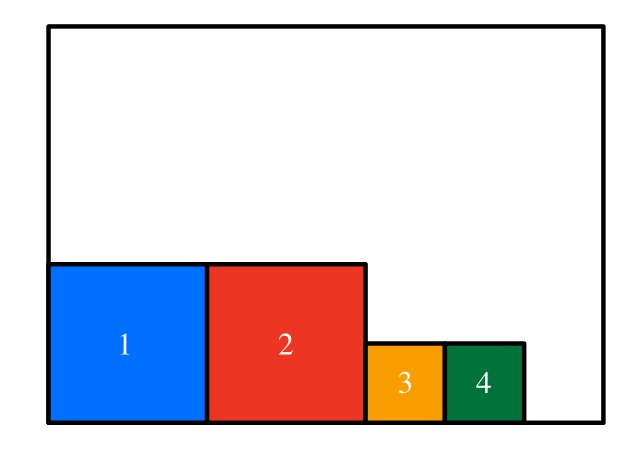
\includegraphics[width=0.5\textwidth]{images/representation.jpg}
    \caption{Final cartons disposition.}
    \label{fig:rep}
\end{figure}

As already said, we decided to generate 30 instances; respectively: 
\begin{itemize}
    \item 5 \textit{easy} instances: a couple of running time seconds;
    \item 20 \textit{medium} instances: a couple of minutes;
    \item 5 \textit{hard} instances: exceeding 5 minutes;
\end{itemize}

Table~\ref{tbl:inst} summarize all principal characteristics of the generated instances.
We will briefly summarize what columns stand for:
\begin{itemize}
    \item $m$: represents the rows of the matrix (room);
    \item $n$: represents the columns of the matrix (room);
    \item $BoxNumber$: number of boxes inside the room;
    \item $MaxDim$: size of the bigger carton inside the room;
\end{itemize}

\begin{longtable}{|c||l|l|c|c|}
\hline
Instance number & m & n & BoxNumber & MaxDim      \\ 
\hline
easy 1           & 3 & 3 & 1         & 2           \\ 
\hline
easy 2           & 3 & 3 & 1         & 2           \\ 
\hline
easy 3           & 3 & 3 & 1         & 2           \\ 
\hline
easy 4           & 4 & 5 & 1         & 3           \\ 
\hline
easy 5           & 3 & 3 & 1         & 2           \\ 
\hline
medium 1         & 5 & 5 & 2         & 3           \\ 
\hline
medium 2         & 5 & 5 & 2         & 3           \\ 
\hline
medium 3         & 5 & 5 & 1         & 3           \\ 
\hline
medium 3         & 5 & 5 & 1         & 3           \\ 
\hline
medium 4         & 5 & 5 & 2         & 3           \\ 
\hline
medium 5         & 5 & 4 & 1         & 3           \\ 
\hline
medium 6         & 4 & 5 & 2         & 3           \\ 
\hline
medium 7         & 4 & 3 & 2         & 2           \\ 
\hline
medium 8         & 4 & 4 & 1         & 3           \\ 
\hline
medium 9         & 5 & 4 & 1         & 3           \\ 
\hline
medium 10        & 4 & 4 & 2         & 3           \\ 
\hline
medium 11        & 4 & 4 & 1         & 3           \\ 
\hline
medium 12        & 4 & 4 & 1         & 3           \\ 
\hline
medium 13        & 5 & 4 & 1         & 3           \\ 
\hline
medium 14        & 4 & 5 & 1         & 3           \\ 
\hline
medium 15        & 5 & 5 & 1         & 3           \\ 
\hline
medium 16        & 4 & 5 & 1         & 3           \\ 
\hline
medium 17        & 4 & 5 & 1         & 3           \\ 
\hline
medium 18        & 4 & 4 & 1         & 3           \\ 
\hline
medium 19        & 4 & 5 & 2         & 3           \\ 
\hline
medium 20        & 5 & 5 & 1         & 3           \\ 
\hline
hard 1           & 8 & 8 & 1         & 4           \\ 
\hline
hard 2           & 8 & 8 & 3         & 4           \\ 
\hline
hard 3           & 8 & 8 & 2         & 4           \\ 
\hline
hard 4           & 8 & 8 & 3         & 4           \\ 
\hline
hard 5           & 7 & 7 & 3         & 4           \\
\hline
\caption{Instances properties}
\label{tbl:inst}
\end{longtable} 






\section{Performance analysis}
We will present benchmarks acquired using both models on all instances. Table~\ref{table:perf} contains all results obtained and times measured. In order:
\begin{itemize}
    \item $best (moves)$: represent the minor number of moves that model's found;
    \item ${time\_found(s)}$: is the time, in seconds, in which the model found the solution in the~\textit{best} column;
    \item ${total\_time(s)}$ is the total time used by the model to explore the computation tree.
\end{itemize}
In cases where~\textit{e} is written it means that computation exceed 5 minutes (even if the correct solution was found). 
As we can see, $ASP\ model$ perfomed better than $MZN$ one almost for every easy and medium instance; the results are opposite in hard instance cases, since in some computations $ASP\ model$ was not even able to find the right minimum. This is probably because the heuristics used perform better with hard instances. A visual representation is given in plots~\ref{fig:bench1},~\ref{fig:bench2}; both use a logarithmic scale on the y-axis since the times interval is slightly big. The first chart represents times taken by the two models to compute the optimal solution, while the second one represents times of total computations of the two models. The upperbound represents $e$, which stands for 300s.
\begin{table}[H] 
\begin{tabular}{l|ccc|ccc|}
\cline{2-7}
                          & \multicolumn{3}{c|}{\textbf{ASP}}                                                         & \multicolumn{3}{c|}{\textbf{MZN}}                                                         \\ \cline{2-7} 
                          & \multicolumn{1}{c|}{best (moves)} & \multicolumn{1}{c|}{time\_found (s)} & total time (s) & \multicolumn{1}{c|}{best (moves)} & \multicolumn{1}{c|}{time\_found (s)} & total time (s) \\ \hline
\multicolumn{1}{|l|}{e1}  & \multicolumn{1}{c|}{2}            & \multicolumn{1}{c|}{0.024}           & 0.024          & \multicolumn{1}{c|}{2}            & \multicolumn{1}{c|}{1.802}           & 1.802          \\ \hline
\multicolumn{1}{|l|}{e2}  & \multicolumn{1}{c|}{2}            & \multicolumn{1}{c|}{0.023}           & 0.023          & \multicolumn{1}{c|}{2}            & \multicolumn{1}{c|}{1.390}           & 2.100          \\ \hline
\multicolumn{1}{|l|}{e3}  & \multicolumn{1}{c|}{2}            & \multicolumn{1}{c|}{0.024}           & 0.024          & \multicolumn{1}{c|}{2}            & \multicolumn{1}{c|}{0.190}           & 1.756          \\ \hline
\multicolumn{1}{|l|}{e4}  & \multicolumn{1}{c|}{1}            & \multicolumn{1}{c|}{0.022}           & 0.022          & \multicolumn{1}{c|}{1}            & \multicolumn{1}{c|}{0.320}           & 0.320          \\ \hline
\multicolumn{1}{|l|}{e5}  & \multicolumn{1}{c|}{2}            & \multicolumn{1}{c|}{0.023}           & 0.023          & \multicolumn{1}{c|}{2}            & \multicolumn{1}{c|}{1.339}           & 1.339          \\ \hline
\multicolumn{1}{|l|}{m1}  & \multicolumn{1}{c|}{8}            & \multicolumn{1}{c|}{0.870}           & e              & \multicolumn{1}{c|}{8}            & \multicolumn{1}{c|}{0.910}           & e              \\ \hline
\multicolumn{1}{|l|}{m2}  & \multicolumn{1}{c|}{5}            & \multicolumn{1}{c|}{0.270}           & e              & \multicolumn{1}{c|}{5}            & \multicolumn{1}{c|}{0.750}           & e              \\ \hline
\multicolumn{1}{|l|}{m3}  & \multicolumn{1}{c|}{3}            & \multicolumn{1}{c|}{0.430}           & 0.486          & \multicolumn{1}{c|}{3}            & \multicolumn{1}{c|}{0.599}           & e              \\ \hline
\multicolumn{1}{|l|}{m4}  & \multicolumn{1}{c|}{5}            & \multicolumn{1}{c|}{0.480}           & 158.699        & \multicolumn{1}{c|}{5}            & \multicolumn{1}{c|}{6.130}           & e              \\ \hline
\multicolumn{1}{|l|}{m5}  & \multicolumn{1}{c|}{3}            & \multicolumn{1}{c|}{0.350}           & 0.397          & \multicolumn{1}{c|}{3}            & \multicolumn{1}{c|}{0.810}           & e              \\ \hline
\multicolumn{1}{|l|}{m6}  & \multicolumn{1}{c|}{4}            & \multicolumn{1}{c|}{11.840}          & 11.899         & \multicolumn{1}{c|}{4}            & \multicolumn{1}{c|}{1.68}            & e              \\ \hline
\multicolumn{1}{|l|}{m7}  & \multicolumn{1}{c|}{4}            & \multicolumn{1}{c|}{1.970}           & 1.995          & \multicolumn{1}{c|}{4}            & \multicolumn{1}{c|}{0.191}           & e              \\ \hline
\multicolumn{1}{|l|}{m8}  & \multicolumn{1}{c|}{3}            & \multicolumn{1}{c|}{0.250}           & 0.285          & \multicolumn{1}{c|}{3}            & \multicolumn{1}{c|}{0.830}           & e              \\ \hline
\multicolumn{1}{|l|}{m9}  & \multicolumn{1}{c|}{2}            & \multicolumn{1}{c|}{0.058}           & 0.060          & \multicolumn{1}{c|}{2}            & \multicolumn{1}{c|}{0.660}           & 4.168          \\ \hline
\multicolumn{1}{|l|}{m10} & \multicolumn{1}{c|}{4}            & \multicolumn{1}{c|}{8.41}            & 9.465          & \multicolumn{1}{c|}{4}            & \multicolumn{1}{c|}{0.890}           & e              \\ \hline
\multicolumn{1}{|l|}{m11} & \multicolumn{1}{c|}{4}            & \multicolumn{1}{c|}{2.18}            & 2.215          & \multicolumn{1}{c|}{2}            & \multicolumn{1}{c|}{0.601}           & e              \\ \hline
\multicolumn{1}{|l|}{m12} & \multicolumn{1}{c|}{3}            & \multicolumn{1}{c|}{0.250}           & 0.289          & \multicolumn{1}{c|}{3}            & \multicolumn{1}{c|}{0.610}           & e              \\ \hline
\multicolumn{1}{|l|}{m13} & \multicolumn{1}{c|}{5}            & \multicolumn{1}{c|}{13.75}           & 13.79          & \multicolumn{1}{c|}{5}            & \multicolumn{1}{c|}{0.760}           & e              \\ \hline
\multicolumn{1}{|l|}{m14} & \multicolumn{1}{c|}{3}            & \multicolumn{1}{c|}{0.370}           & 0.411          & \multicolumn{1}{c|}{3}            & \multicolumn{1}{c|}{0.680}           & e              \\ \hline
\multicolumn{1}{|l|}{m15} & \multicolumn{1}{c|}{4}            & \multicolumn{1}{c|}{3.87}            & 3.914          & \multicolumn{1}{c|}{4}            & \multicolumn{1}{c|}{0.760}           & e              \\ \hline
\multicolumn{1}{|l|}{m16} & \multicolumn{1}{c|}{4}            & \multicolumn{1}{c|}{3.10}            & 3.147          & \multicolumn{1}{c|}{4}            & \multicolumn{1}{c|}{0.630}           & e              \\ \hline
\multicolumn{1}{|l|}{m17} & \multicolumn{1}{c|}{2}            & \multicolumn{1}{c|}{0.054}           & 0.060          & \multicolumn{1}{c|}{2}            & \multicolumn{1}{c|}{0.960}           & 3.631          \\ \hline
\multicolumn{1}{|l|}{m18} & \multicolumn{1}{c|}{3}            & \multicolumn{1}{c|}{0.250}           & 0.283          & \multicolumn{1}{c|}{3}            & \multicolumn{1}{c|}{0.566}           & e              \\ \hline
\multicolumn{1}{|l|}{m19} & \multicolumn{1}{c|}{5}            & \multicolumn{1}{c|}{17.00}           & 207.847        & \multicolumn{1}{c|}{5}            & \multicolumn{1}{c|}{35.290}          & e              \\ \hline
\multicolumn{1}{|l|}{m20} & \multicolumn{1}{c|}{3}            & \multicolumn{1}{c|}{0.440}           & 0.488          & \multicolumn{1}{c|}{3}            & \multicolumn{1}{c|}{0.680}           & e              \\ \hline
\multicolumn{1}{|l|}{h1}  & \multicolumn{1}{c|}{6}            & \multicolumn{1}{c|}{14.15}           & e              & \multicolumn{1}{c|}{6}            & \multicolumn{1}{c|}{2.810}           & e              \\ \hline
\multicolumn{1}{|l|}{h2}  & \multicolumn{1}{c|}{48}           & \multicolumn{1}{c|}{112.10}          & e              & \multicolumn{1}{c|}{16}           & \multicolumn{1}{c|}{11.470}          & e              \\ \hline
\multicolumn{1}{|l|}{h3}  & \multicolumn{1}{c|}{12}           & \multicolumn{1}{c|}{123.65}          & e              & \multicolumn{1}{c|}{12}           & \multicolumn{1}{c|}{108.150}         & e              \\ \hline
\multicolumn{1}{|l|}{h4}  & \multicolumn{1}{c|}{37}           & \multicolumn{1}{c|}{267.31}          & e              & \multicolumn{1}{c|}{19}           & \multicolumn{1}{c|}{214.000}         & e              \\ \hline
\multicolumn{1}{|l|}{h5}  & \multicolumn{1}{c|}{9}            & \multicolumn{1}{c|}{146.00}          & e              & \multicolumn{1}{c|}{9}            & \multicolumn{1}{c|}{14.790}          & e              \\ \hline
\end{tabular}
\caption{Benchmarks}
\label{table:perf}
\end{table}

\begin{figure}[H]
	\centering
	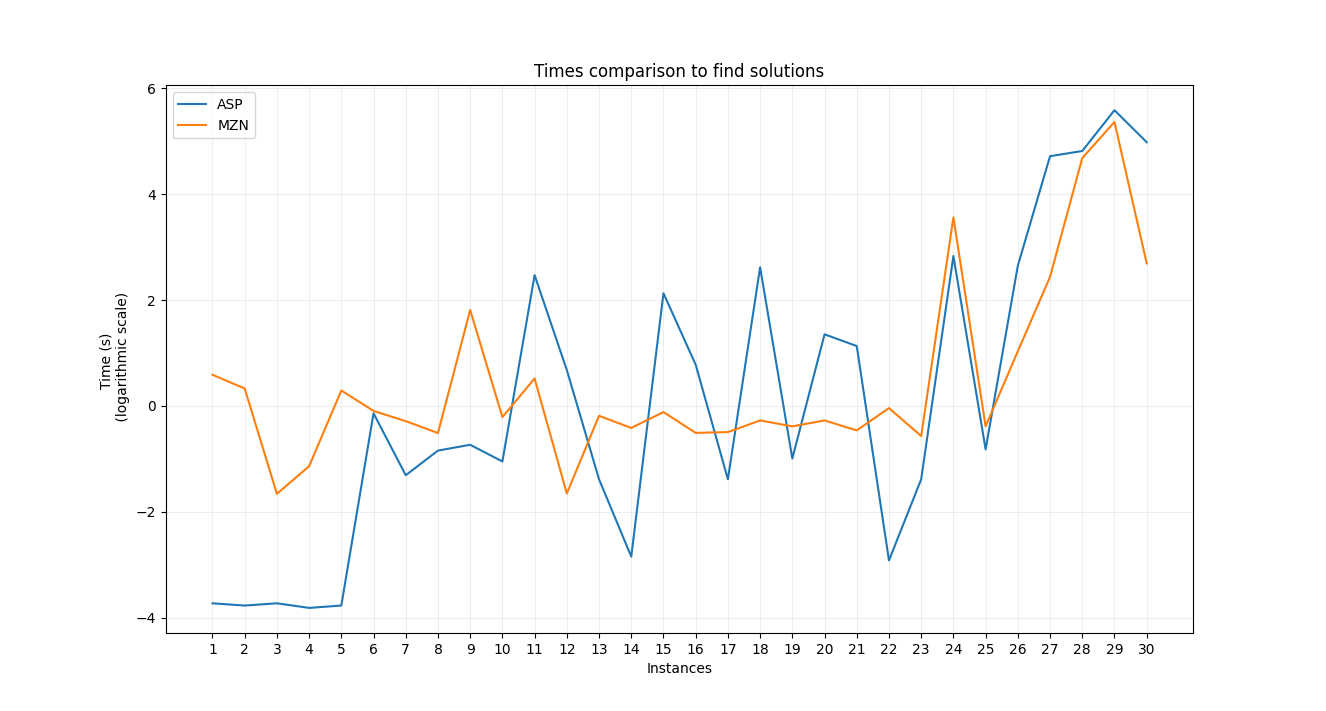
\includegraphics[width=0.99\textwidth]{images/Figure_1.png}
    \caption{Benchmarks of solutions time, in logarithmic scale.}
    \label{fig:bench1}
\end{figure}

\begin{figure}[H]
	\centering
	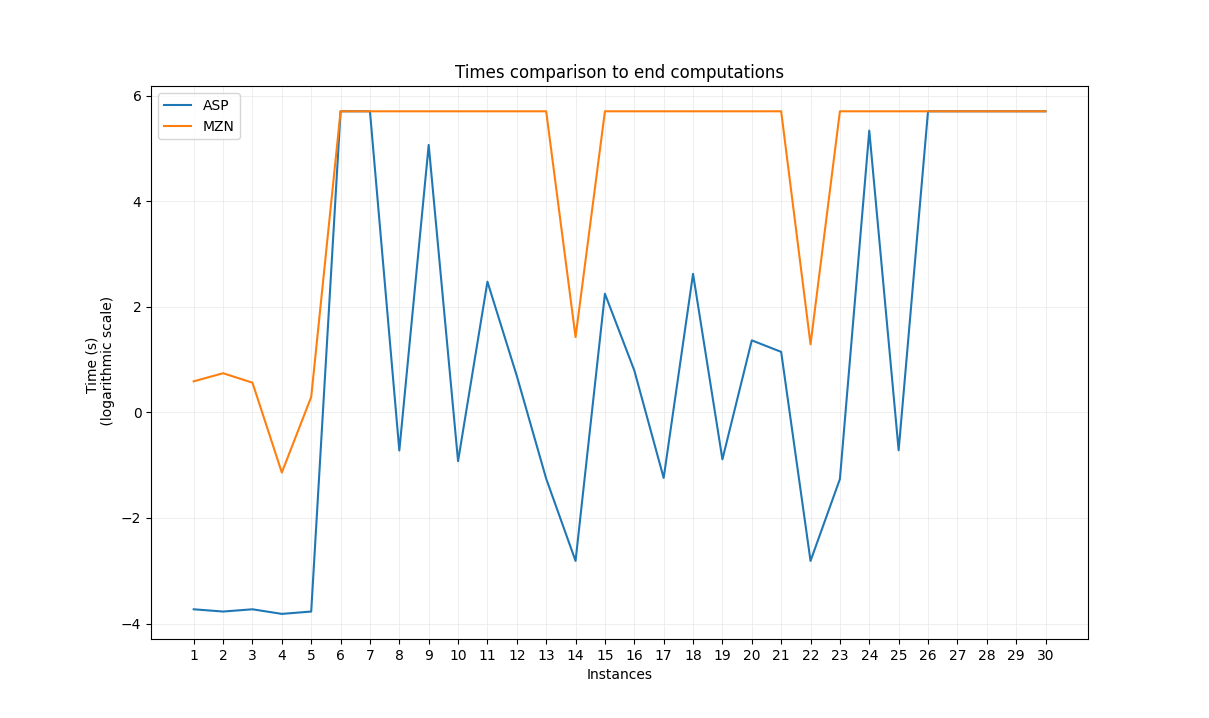
\includegraphics[width=0.99\textwidth]{images/total computation.png}
    \caption{Benchmarks of computations time, in logarithmic scale.}
    \label{fig:bench2}
\end{figure}

\bibliography{thud}
\end{document}
